\documentclass[a4paper]{scrreprt}
 
\usepackage[german]{babel}
\usepackage[utf8]{inputenc}
\usepackage[T1]{fontenc}
\usepackage{ae}
\usepackage[bookmarks,bookmarksnumbered]{hyperref}
\usepackage{graphicx}
\graphicspath{ {Images/} }
 
\begin{document}
 
    \begin{flushright}
        
\includegraphics[scale = 0.7]{kit-logo.jpg}\\[0.5cm]
        % 
\includegraphics[scale = 1]{teco.jpg}
    \end{flushright}
    % 
\includegraphics[scale = 0.5]{kit-logo.jpg} \hspace{4cm} 
\includegraphics[scale = 1]{teco.jpg}
    \vspace*{2cm} 

    \begin{center} \large 
    
        Praxis der Softwareentwicklung
        \vspace * {1.5cm}

        {\bf \huge Mind Rate}
		
        \vspace*{1cm}
		
        {\bf \large Ein interaktives Feedbacksystem f\"ur psychologische Untersuchungen nach Experience-Sampling-Method}
        \vspace*{1cm}

        {\large Pflichtenheft}
        \vspace*{2cm}

        Shanshan Du, Yi Ge, Renhan Lou, Ruoheng Ma, Haobin Tan
        \vspace*{1cm}

        02. Dezember 2016
        \vspace*{2.5cm}


        Betreuung: Anja Exler, Erik Psescara\\[1cm]
        Technology f\"ur Pervasive Computing\\[0.5cm]
        Karlsruher Institut für Technologie
    \end{center}
 
    % Die abstract-Umgebung kann bei Bedarf aus dem Pflichtenheft entfernt werden
    % \begin{abstract}
    %     Dies ist ein beispielhaftes Pflichtenheft in \LaTeX. Das Pflichtenheft
    %     beschreibt in konkreter Form, wie der Auftragnehmer die Anforderungen des
    %     Auftraggebers zu lösen gedenkt - das sogenannte wie und womit. Der Auftraggeber
    %     beschreibt vorher im Lastenheft möglichst präzise die Gesamtheit der
    %     Forderungen - was er entwickelt oder produziert haben möchte. Erst wenn der
    %     Auftraggeber das Pflichtenheft akzeptiert, sollte die eigentliche Arbeit beim
    %     Auftragnehmer beginnen.
    %     \vspace{1cm}
 
    %     Quelle: \url{http://de.wikipedia.org/wiki/Pflichtenheft} und Lehrbuch der
    %     Objektmodellierung von Heide Balzert
    %     \vspace{0.5cm}
 
    %     Quellcode: \url{http://www.karllorey.de/informatik-studium/vorlesungen/softwarepraktikum/pflichtenheft-in-latex/}
    % \end{abstract}
 
    % Platzierung des Inhaltsverzeichnisses
    \tableofcontents
 
    \chapter{Zielbestimmung}
    % Dieses Kapitel dient der Bestimmung von Zielen und nicht für deren Verwendung
    % notwendige Funktionen.
        Die Firma soll durch das Produkt in die Lage versetzt werden, psychologische Untersuchungen nach Experience-Sampling-Method\footnote{\url{https://en.wikipedia.org/wiki/Experience_sampling_method}} (ESM) durchzuf\"uhren und Feedbacks der Untersuchungen zu erhalten.
 
 
        \section{Musskriterien}
            % Musskriterien: Für das Produkt unabdingbare Leistungen, die in jedem Fall
            % erfüllt werden müssen \footnote{gezwungen sein, etwas zu tun (Dies ist eine
            % beispielhafte Fußnote).}. Das System ist ohne diese Funktionen für seinen
            % gedachten Zweck nicht einsetzbar.

            \subsection{Verwalten von Teilnehmer der Untersuchung}
                \begin{itemize}
                    \item Probandsstatus erfassen (z.B. Name, Email, Alter, Geschlecht, Beruf)
                    \item Registrieren, Anmelden f\"ur Beteiligung der Untersuchung
                \end{itemize}
            
            \subsection{Verwalten der Frageb\"ogen}
                \begin{itemize}
                    \item Erstellen, \"Andern von Untersuchungsfragen
                    \item Erstellen, \"Andern von Scale und Optionen der Antworten
                    \item Setzen, \"Andern von G\"ultigkeitszeitbereich der Untersuchungsfragen
                    \item Setzen, \"Andern von H\"aufigkeit der Notifikationen zur Antworten
                    \item Ausw\"ahlen von Prob\"ande nach Bedarf
                \end{itemize}
            
            \subsection{Antwort auf Untersuchungsfragen}
                \begin{itemize}
                    \item regelm\"assige Notifikation zur Antworten
                    \item Untersuchungsfragen beantworten
                \end{itemize}
                
            \subsection{Verwalten von Antworten}
                \begin{itemize}
                    \item lokales Speichern von Antworten
                    \item Protokollieren von Zeitpunkt der Antwort
                    \item Hochladen von Antworten auf den Server
                \end{itemize}
            
            \subsection{Erfassen von Ergebnisse der Untersuchung}
                \begin{itemize}
                    \item Exportieren von Daten  
                \end{itemize}
 
        \section{Wunschkriterien}
            % Kannkriterien: Die Erfüllung der Kannkriterien ist erwünscht, jedoch nicht
            % unbedingt notwendig. Sie sollten nur angestrebt werden, falls noch ausreichend
            % Kapazitäten vorhanden sind.
            \begin{itemize}
                \item Emailbest\"atigugn beim (erfolgreichen) Anmelden
                \item Erm\"oglichen von ``angemeldet bleiben"
                \item Erzeugen von verschiedenen (Statistik-)Diagramme f\"ur hochgeladene Daten (z.B. S\"aulendiagramm, Kreisdiagramm) 
                \item Unterst\"utzen von unterschiedlichen Sprachen
                \item Wechseln von Theme der Anwendung
            \end{itemize}
 
        \section{Abgrenzungskriterien}
            % Abgrenzungskriterien: Diese Kriterien sollen bewusst nicht erreicht werden.
            \begin{itemize}
                \item Keine verteilte Datenbank, keine Echtzeitanforderungen, keine synchronisierten Datenbankzugriffe
                \item Keine Unterst\"utzung f\"ur iOS
            \end{itemize}
 
    \chapter{Produkteinsatz}
        Das Produkt dient zur Sammlung der Versuchsdaten aus psychologischen Versuchen nach ESM. Damit bietet sie für Versuchsleiter eine Lösung, ESM-Versuchen durchzuführen. Diese Tätigkeit soll zusätzlich im Internet und auf dem Smartphone möglich sein.
 
        \section{Anwendungsbereiche}
            \begin{itemize}
                \item Akademischer / Sozialwissenschaftlicher Anwendungsbereich
                \item Statistischer Anwendungsbereich
            \end{itemize}
 
        \section{Zielgruppen}
            \begin{itemize}
                \item Versuchsleiter eines ESM-Versuchs
                \item Teilnehmer des Versuchs
            \end{itemize}
 
        \section{Betriebsbedingungen}
            \begin{itemize}
                \item Versuchsleiter: Büroumgebung
                \item Versuchsteilnehmer: im alltäglichen Leben aufs Smartphone
                \item Betriebszeit rund um die Uhr, läuft unbeaufsichtigt
            \end{itemize}
 
    \chapter{Produktumgebung}
        Eine Client-Server Architektur mit 2 Client-Typen: der Web-Client für Versuchsleiter und der Smartphone-Client für Versuchsteilnehmer

        \section{Software}
            \begin{itemize}
                \item Serverseite
                    \begin{itemize}
                        \item  Läuft auf Linux
                        \item Alle Softwares der Serverseite werden durch Docker verpackt
                        \item Datenbank: SQLite, verwaltet durch das Django-Framework
                        \item Programmiersprache: Python 3
                        \item Web server: Nginx
                    \end{itemize}
                \item Clientseite
                    \begin{itemize}
                        \item Web-Client\\
                             Web-Browser, Referenzstandard Google Chrome 54
                        \item  Smartphone-Client\\
                             Android, Referenzstandard Android 7.1 Nougat
                    \end{itemize}
            \end{itemize}
 
        \section{Hardware}
            \begin{itemize}
                \item Serverseite\\
                    Leistungsstarke Standardrechner
                \item  Web-Client\\
                    Standardrechner
                \item Smartphone-Client\\
                    Standardsmartphone
            \end{itemize}

    \chapter{Funktionale Anforderungen}
 
        \begin{itemize}
            \item /F10/Anmelden oder Registrieren der Leiter
            	\par Registrieren: Der Leiter soll sich zuerst in dem Online-Verwaltungssystem mit seinem Email-Adresse registrieren. Dabei soll ein gültiges Passwort zweimal eingeben. Wenn ein neues Konto in dem Datenbank erstellt ist, soll der Leiter ein Bestätigungsemail empfangen.\par
Anmelden: Wenn ein Konto schon vorhanden ist, kann ein Leiter sich damit anmelden.
        \end{itemize}
        
        \begin{itemize}
            \item /F20/Vergessenes Passwort neu zu setzen
            	\par Wenn ein Leiter sein Passwort vergessen hat, kann er auf “Passwort Vergessen” klicken und in der weitergeleiteten Seite seine Email-Adresse eingeben. Danach empfängt er ein Bestätigungsemail mit einem Link. Durch dieses Link ist er in die “Passwort neu setzen” Seite weitergeleitet und sein neues Passwort wird in dem Datenbank gespeichert.

        \end{itemize}
        
        \begin{itemize}
            \item /F30/Erstellung eines Fragebogens (Inhalt, regelmäßige Sendungszeit, Zeitzone, gültiger Zeitraum für die Antworten)

            	\par Nach der Anmeldung ist der Leiter in die Verwaltungsseite geleitet. Da kann er Fragebogen erstellen und die Sendungszeit festlegen. Es gibt dabei noch eine Zeitzone-Option. Mit dieser Option kann der Leiter sich entscheiden, ob das Fragebogen abgesehen von Zeitzonen um dieselbe Uhrzeit geschickt wird oder um dieselbe Zeit je nach den Zeitzonen. Außerdem kann der Leiter festlegen, wie lange ist der Zeitraum für eine gültige Antwort.
                
        \end{itemize}
        
        \begin{itemize}
            \item /F40/Verwaltung der persönlichen Daten von Probanden

            	\par Der Leiter kann die persönlichen Daten der Probanden (Email-Address, Name, Alter, Geschlecht usw.) hinfügen, löschen, abfragen und ändern.

        \end{itemize}
        
        \begin{itemize}
            \item /F50/Kontrolle durch Metadata
            	\par Der Leiter kann das Metadata über seine Fragebogen sehen.

        \end{itemize}
        \begin{itemize}
            \item /F60/Exportieren von Daten und Metadata
            	\par Der Leiter kann alle Antworten und die Metadata (z.B. Anzahl von Teilnehmer, Verhältnis zwischen positiven und negativen Antworten) hinsichtlich seiner allen Fragebogen in Form von CSV exportieren.

        \end{itemize}
        \begin{itemize}
            \item /F70/Anmelden oder Registrieren der Probanden

            	\par Registrieren: Die Probanden sollen sich in der App zuerst registrieren. Dabei soll ein gültiges Passwort zweimal eingeben. Wenn ein neues Konto in dem Datenbank erstellt ist, soll der Proband ein Bestätigungsemail empfangen.
                \par Anmelden: Wenn ein Konto schon vorhanden ist, kann ein Proband sich damit anmelden.



        \end{itemize}
        \begin{itemize}
            \item /F80/Antworten eines Fragebogens

            	\par Nachdem der Leiter einen Fragebogen den Probanden gesandt hat, sollen die Probanden eine Notifikation empfangen. Das Fragebogen soll in der App gezeigt werden. Danach werden die Fragen des Fragebogens geantwortet.
                \par
Wenn die Probanden auf alle Fragen geantwortet und auf “Senden“ geklickt haben, werden diese Ergebnisse des Fragebogens zuerst lokal automatisch gespeichert. 


        \end{itemize}
        \begin{itemize}
            \item /F90/Versendung der Antworten eines Fragebogens

            	\par Die lokal gespeicherten Ergebnisse werden unter Netzwerkverbindung zu dem Server geschickt. Falls keine Netzwerkverbindung vorhanden ist, soll die App dazu nichts machen. Sobald die Netzwerkverbindung wieder da ist, soll die App versuchen, die Ergebnisse zu senden.


        \end{itemize}
 
    \chapter{Produktdaten}
        \section{Versuchsleiterdaten}
            \begin{itemize}
                \item /D10/ Über einen Versuchsleiter sind folgende Daten zu speichern:
                    \par Name (Anrede, Titel, Vorname, Nachname), Mailadresse (als Kontonummer im System)
                    
                \item /D20/ Macht ein Versuchsleiter Versuche, dann sind folgende Daten zu speichern:
                    \par Versuchsummern der zum Versuchsleiter gehörten Versuchen
            \end{itemize}
            
        \section{Versuchsteilnehmerdaten}
            \begin{itemize}
                \item /D30/ Über einen Versuchsteilnehmer sind folgende Daten zu speichern:
                    \par Name (Anrede, Titel, Vorname, Nachname), Mailadresse (als Kontonummer im System), Telefonnummer, demographische Daten (Geburtsdatum, Beruf, Geschlecht), Notiz
                
                \item /D40/ Nimmt ein Versuchsteilnehmer an Versuchen teil, dann sind folgende Daten zu speichern:
                    \par Versuchsnummern der daran beteiligten Versuchen
            \end{itemize}
            
        \section{Versuchsdaten}
            \begin{itemize}
                \item /D50/ Über einen Versuch sind folgende Daten zu speichern:
                    \par Versuchsnummer, Versuchsname, Anfangs- und Endedatum, Mailadresse der Versuchsleiter, Notiz
                    
                \item /D60/ Hat ein Versuch Teilnehmer, dann sind folgende Daten zu speichern:
                    \par Mailadressen der Versuchsteilnehmer
                    
                \item /D70/ Hat ein Versuch Fragen, dann sind folgende Daten zu speichern:
                    \par Fragenummer der Fragen
            \end{itemize}
            
        \section{Fragendaten}
            \begin{itemize}
                \item /D80/ Über eine Versuchsfrage sind folgende Daten zu speichern:
                    \par Fragenummer, Fragetyp, Inhalt der Frage, Versuchsnummer des zugehörigen Versuchs
                    
                \item /D90/ Wird eine Frage im Versuch erscheinen, dann sind folgende Daten zu speichern:
                    \par Erscheinungskriterium, Abgabetermin
                    
                \item /D100/ Wird eine Frage von Versuchsteilnehmern beantwortet, dann sind folgende Daten zu speichern:
                    \par Mailadressen der Antwortgeber, Abgabezeit der Antworten, Inhalt der Antworten
            \end{itemize}
 
   \chapter{Nichtfunktionale Anforderungen}
        \begin{itemize}
            \item /NF10/Reaktionszeit

            	\par Die App darf nicht mehr als \_ Sekunden Reaktionszeit haben und die Ladezeit muss unter \_ Sekunden liegen.

                
        \end{itemize}
 
        \begin{itemize}
            \item /NF20/Registrierung

            	\par Die Registrierung erfolgt unter Angabe einer E-Mail Adresse und einem Passwort.
                
        \end{itemize}
        \begin{itemize}
            \item /NF30/Passwort

            	\par Passwörter müssen mindestens 6-stellig sein. Die App kann angemeldet bleiben.

                
        \end{itemize}
        \begin{itemize}
            \item /NF40/Globalisierung

            	\par Die App ist auf Deutsch und Englisch verfügbar.

                
        \end{itemize}
        \begin{itemize}
            \item /NF50/Daten speichern

            	\par Die Antworten jedes Fragebogens von den Probanden muss ins Handy gespeichert werden.

                
        \end{itemize}
        \begin{itemize}
            \item /NF60/Größe der App

            	\par Die App darf nicht mehr als \_ Mb auf dem Handy benötigen.


                
        \end{itemize}
        \begin{itemize}
            \item /NF70/Integration ins Google Play Store

            	\par Die App soll ins Google Play Store integriert werden.


                
        \end{itemize}
 
    % \chapter{Benutzungsoberfläche}
    %     Benutzungsoberfläche: grundlegende Anforderungen, Zugriffsrechte
 
        \begin{figure}[ht]
            \centering
            \rule{8cm}{6cm}
            \caption{Dies könnte ein Bild der Benutzungsoberfläche sein}
        \end{figure}

    \chapter{Globale Testfälle}

    \chapter{Systemmodelle}

        \section{Szenarien}

        \section{Anwendungsf\"alle}

            \newpage
            \subsection{Anwendungsfalldiagramm} 
                \vspace{0.2cm}
                \begin{center}
                    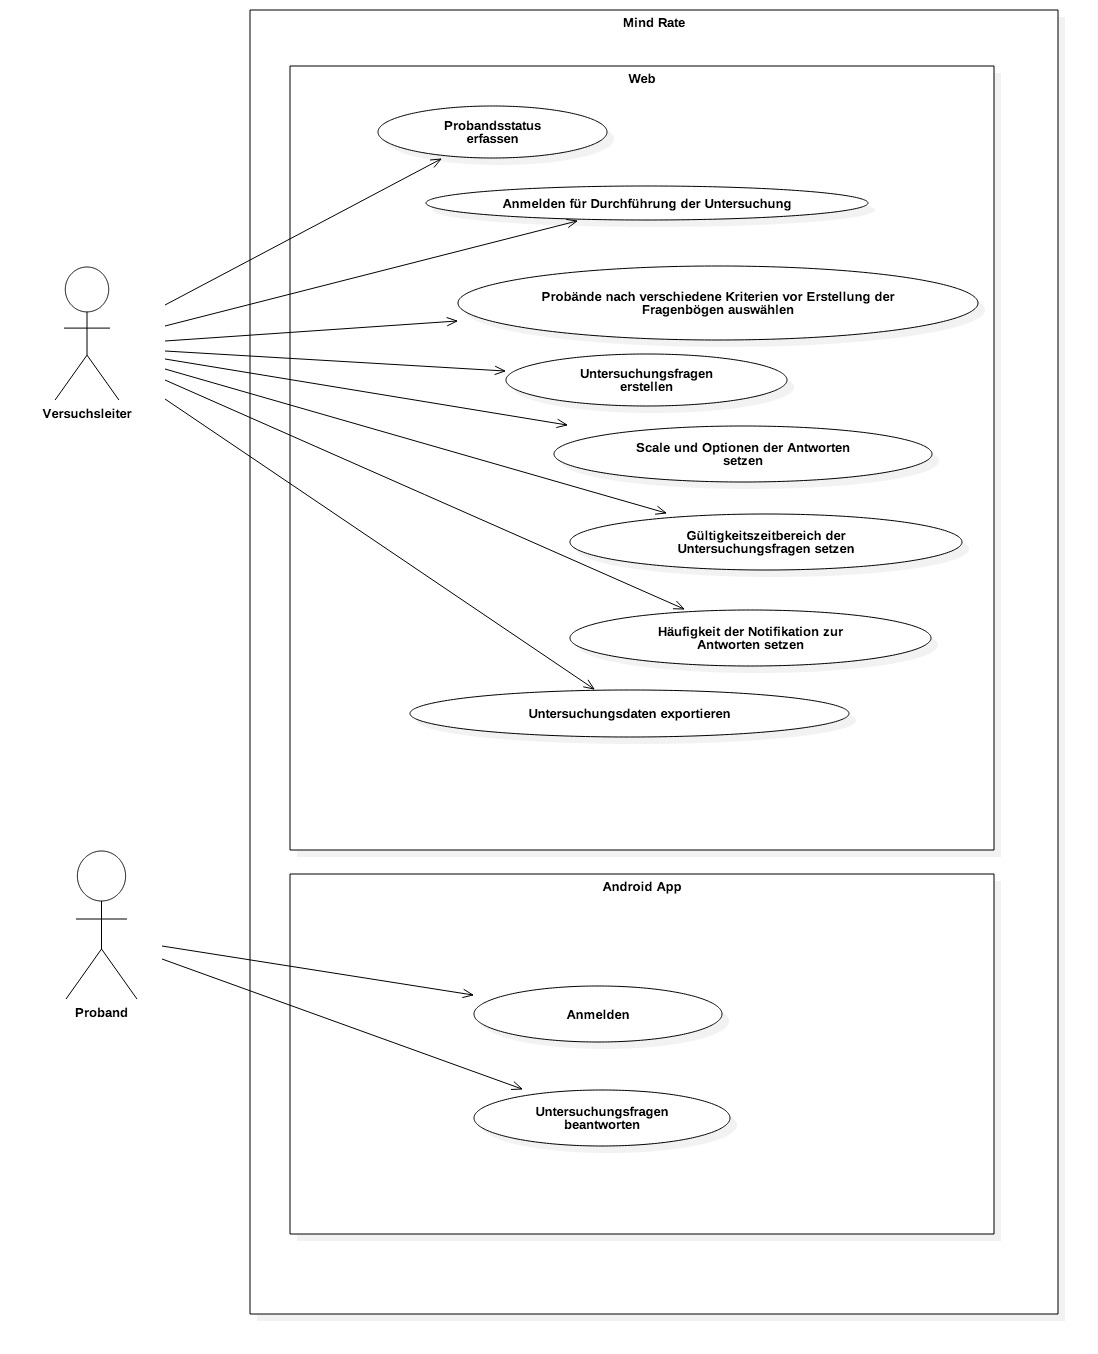
\includegraphics[scale = 0.4]{UseCaseDiagram1.jpg}
                \end{center}

        \newpage
        \section{Benutzerschnittstelle}
 
    \chapter{Qualitätsziele}
        Qualiätsziele: Allgemeine Ziele sind meistens Änderbarkeit und Wartbarkeit.
        Ziele sollten jedoch grundsätzlich messbar, spezifisch und relevant sein.
 
    \chapter{Glossar}
 
    % Abbildungsverzeichnis
    \listoffigures
 
\end{document}
